\section{Control Station}\label{sec:implementation_control_station}

The control station as mentioned in \cref{sec:design_control_station} is the station that monitors the \gls{uav} in real-time. It is responsible for receiving telemetry data from the \gls{uav} and sending commands to update its flight plan. The control station is also responsible for creating a geofence around the area of operation, monitoring the \gls{uav}'s position and altitude in real-time, and tracking multiple \glspl{uav} simultaneously.

The control station is composed of a ground control station running a waypoint planning software, in this case, the Mission Planner software \autocite{ardupilotMissionPlanner}, see \cref{fig:control_station_radiocontroller}. The radiocontroller is connected to the telemetry module of the \gls{uav} to send commands and receive telemetry data via the \gls{rf} module. The mission planner software is connected to the radiocontroller via a \gls{wifi} connection to receive telemetry data and send commands to the \gls{uav} by relaying them through the radiocontroller.

\begin{figure}
  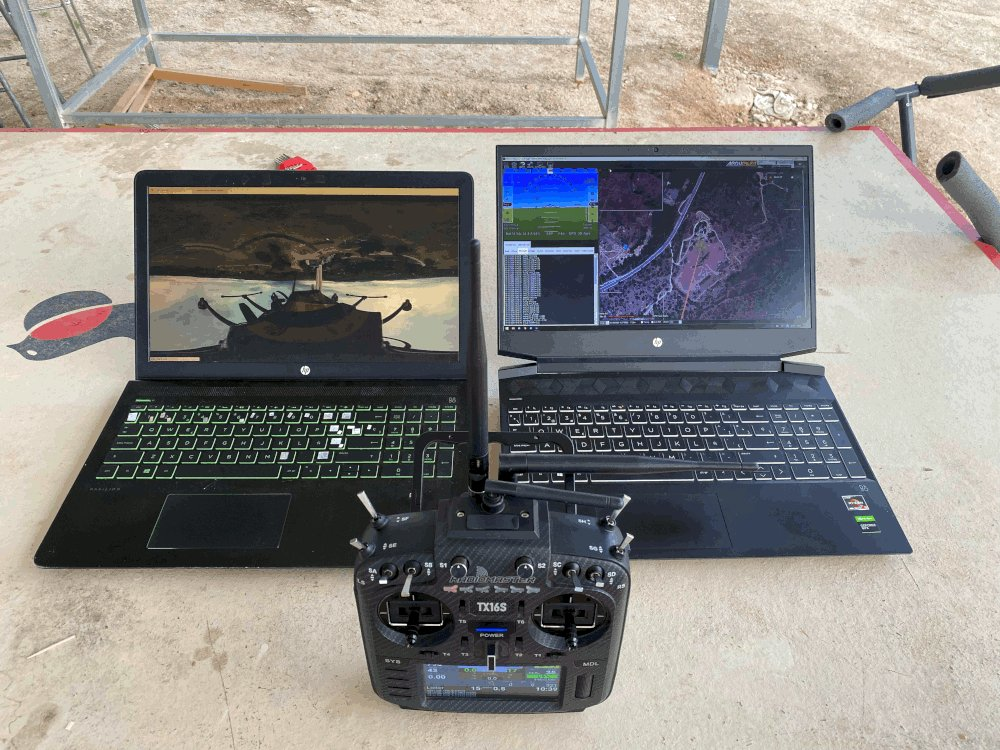
\includegraphics[width=\linewidth]{control_station_radiocontroller.jpg}
  \caption{Control Station setup. On the right, the Mission Planner software running on a laptop. On the left, the reconnaissance platform receiving the video feed. On the bottom center, the RadioMaster TX16S radio controller.}\label{fig:control_station_radiocontroller}
\end{figure}

% Local Variables:
% jinx-local-words: "ardupilotMissionPlanner uav"
% End:
